\documentclass{article}

\usepackage[utf8]{inputenc}
\usepackage{amsmath, amssymb}
\usepackage{graphicx}

\title{ASTR 400B HW7 \\ Analysis and Answers}
\author{Avichal Kaul}
\date{23/03/23}

\begin{document}
	\maketitle

\begin{figure}[htpb]
	\centering
	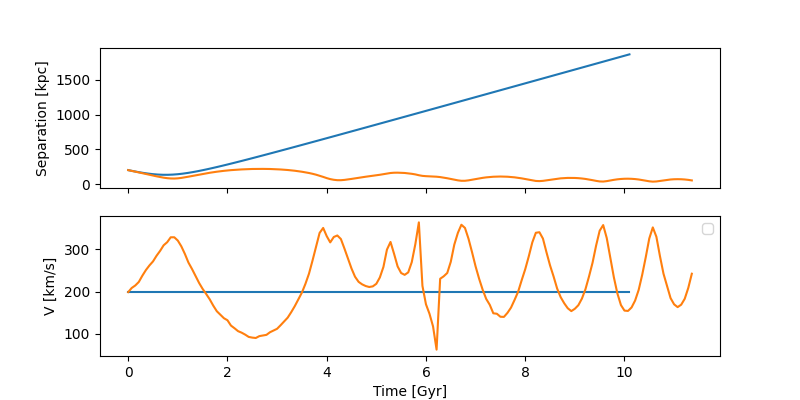
\includegraphics[width=1\textwidth]{../fig.png}
	\caption{M31 Orbit HW7 vs HW6}
	\label{fig:}
\end{figure}	
\begin{enumerate}
	\item The plots are very different. While one seems to show many close encounters, the other only shows one close encounter, and then the two galaxies move away on a long arc before coming back together.
	\item The dynamical friction from the Dark Matter Halo seems unaccounted for. Could it be the reason we don't see a more dramatic interaction at the start?
	\item We could include the MW by creating a similar class for MW's effect on M31, and simply incorporating it into the calculation. Though, this seems like a naive approach, as it does not consider M33's effect on the MW. 
\end{enumerate}
\end{document}
